\subsection{4-2-4 Encoder} 

%============================================================
\subsubsection{Two learning rate} 
\label{sec:tlr-auto4} 
\ref{sec:datasets-auto4} 
%======== (3D) L1 x L2 x epochs =========
%======== (3D) L1 x L2 x patSuccF =========
\begin{figure}[H]
  \centering
  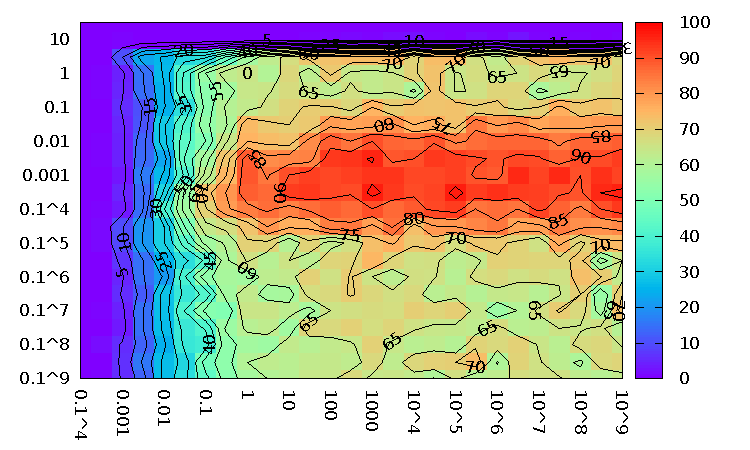
\includegraphics[width=0.48\textwidth]{img/tlr-auto4-success.pdf}   
  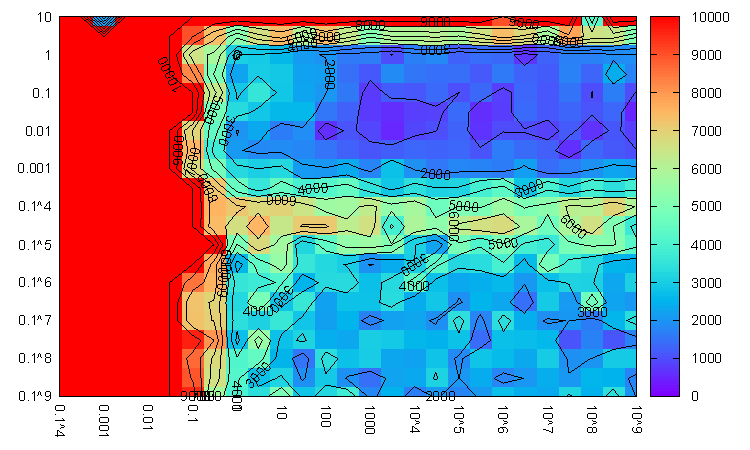
\includegraphics[width=0.48\textwidth]{img/tlr-auto4-epoch.pdf}     
  \caption{TLR success and convergence on the \emph{4-2-4 Encoder} task with $\lambda_h=0.0002$, $\lambda_v=500$, $\sigma = 2.3$ and $\mu = 0.0$.}
  \label{fig:results-tlr-auto4-performance}
\end{figure}

%======== (2D) best TLR on ALL_SUCC x epoch (std-dev) ==========
\begin{figure}[H]
  \centering
  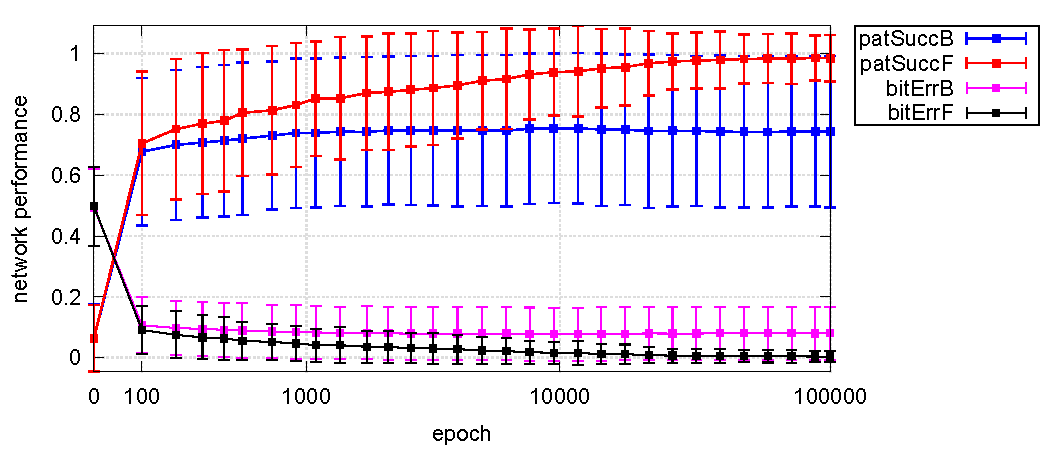
\includegraphics[width=0.5\textwidth]{img/tlr-best-perf.pdf}      
  \caption{TLR success evolution for the \emph{4-2-4 Encoder} task.}
  \label{fig:results-tlr-auto4-epoch} 
\end{figure}

%============================================================
\subsubsection{Comparison} 
\label{sec:tlr-auto4-cmp} 

For all our models \ref{sec:sim-our} and \ref{sec:sim-exp} tested on the 4-2-4 encoder task~\ref{sec:datasets-auto4} TLR~\ref{sec:our-tlr} had the best success rate. 

For TLR, BAL, GeneRec, BP, CHL, other learning rules
\label{sec:our-learning-rules}
It's possible for both BAL \ref{sec:models-bal} and GeneRec \ref{sec:models-generec} to try different learning rules mentioned in \ref{sec:models-generec-modifications}. We will denote such models as \emph{BAL-sym} and \emph{GR-sym} for symmetry perserving rule~\ref{eq:models-generec-learning-rule-sym}; \emph{BAL-mid} and \emph{GR-mid} for midpoint rule~\ref{eq:models-generec-learning-rule-mid} and \emph{BAL-chl} and \emph{GR-chl} for CHL rule~\ref{eq:models-generec-learning-rule-chl} but none of them worked. 
\label{sec:our-bal-sym} 
\emph{Symmetric BAL (SymBAL)} is inspired by the necessary condition for convergence of GeneRec \citep{o1996bio} we set symmetric weights $W^{IH} = (W^{HI})^T$ and $W^{HO} = (W^{OH})^T$. 

\begin{table}[H] 
  \centering
    \begin{tabular}{|l|l|l|l|l|}
    \hline
    Algorithm&$\lambda$&Success&Epcs&SEM \\
    \hline
    BP&2.4&100&60&5.1\\
    \hline
    AP&2.8&100&54&3.6\\
    \hline
    GR&0.6&90&418&28\\
    \hline
    GR Sym&1.4&56&88&2.9\\
    \hline
    GR Mid&2.4&92&60&3.4\\
    \hline
    CHL&1.2&56&77&1.8\\
    \hline
    BAL&0.9&65& &\\
    \hline
    BAL TLR&0.0002 | 500&93.12&5845.01&1.52e+08\\
    \hline
    BAL TLR 1000 can&0.0002 | 500&99.86&150.417&5,070,000\\
    \hline
    BAL Recirc&0.7&34&10000&\\
    \hline
    \end{tabular}
  \caption{Comparing performance of different models on the \emph{4-2-4 encoder} task.} 
  \label{tab:results-cmp-auto4}
\end{table}

TODO note that one epoch computation is not same for different models, for instance GeneRec needs to settle in the iterative approach 

%============================================================
\subsubsection{Hidden activations}
\ref{sec:our-hidden-activation}  

%===== TODO hidden activation timelines with commentaries (for TLR, BAL, GeneRec) 
% 2x success, 2x error (wrong settle, divergence) 

\begin{figure}[H]
  \centering
  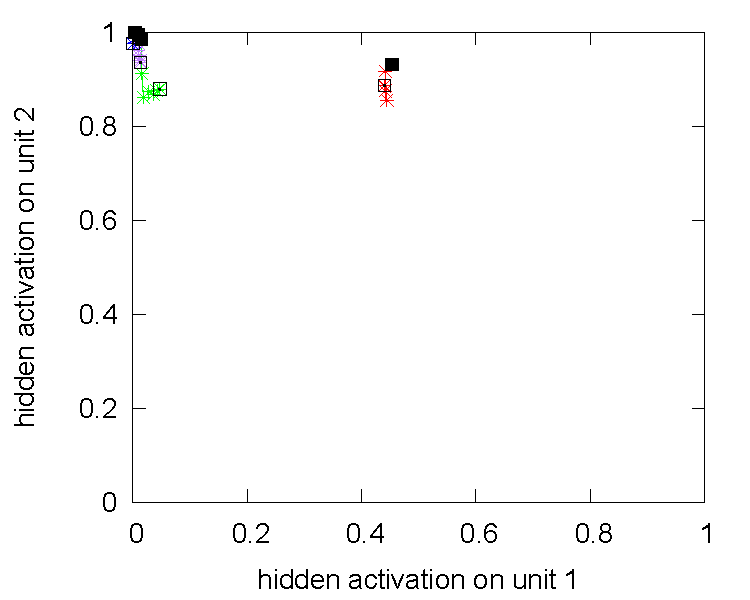
\includegraphics[width=0.48\textwidth]{img/hid-bal-bad-init.pdf}  
  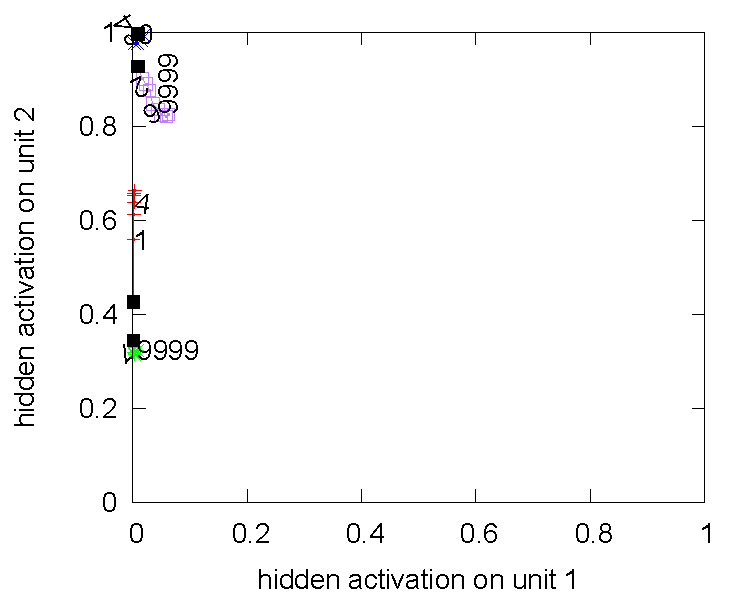
\includegraphics[width=0.48\textwidth]{img/hid-bal-bad-convex.pdf}  \\
  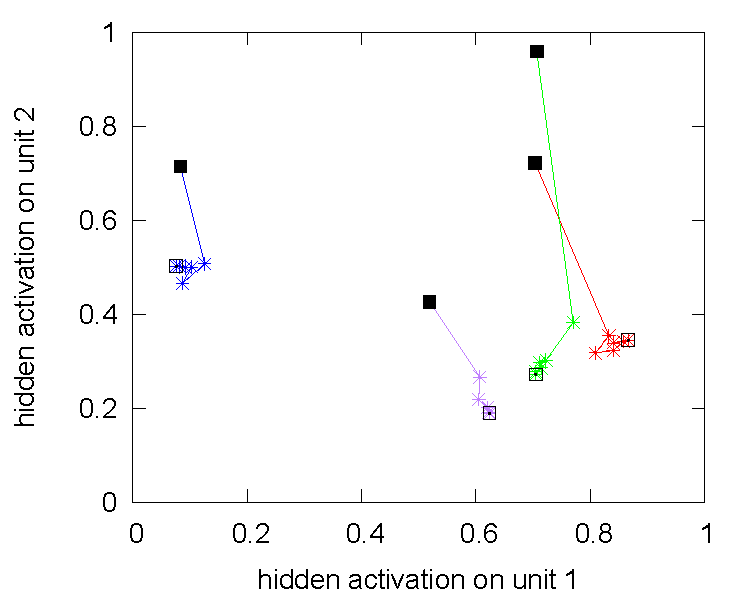
\includegraphics[width=0.48\textwidth]{img/hid-bal-bad-step.pdf}  
  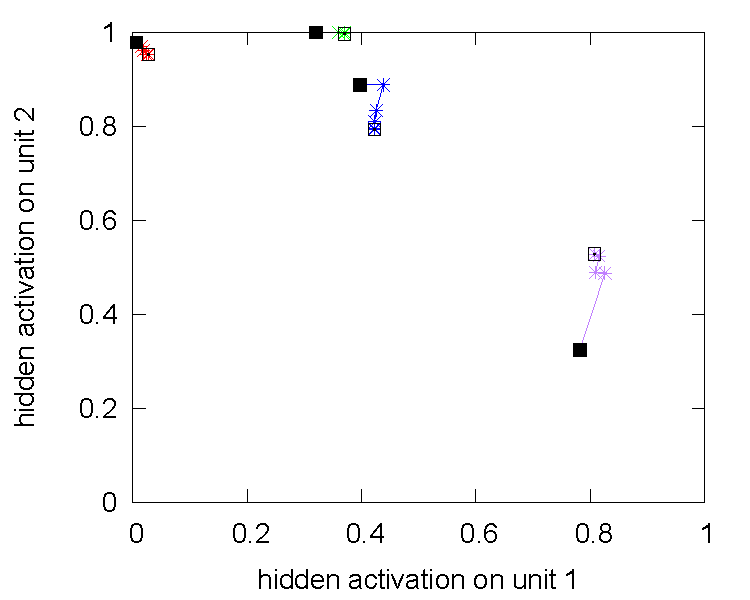
\includegraphics[width=0.48\textwidth]{img/hid-bal-bad-stagnation.pdf}  \\
  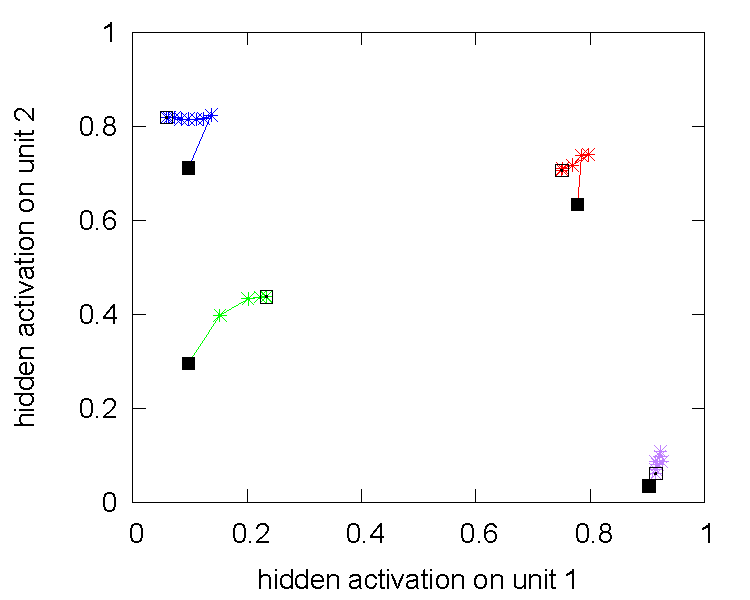
\includegraphics[width=0.48\textwidth]{img/hid-bal-good-init.pdf}  
  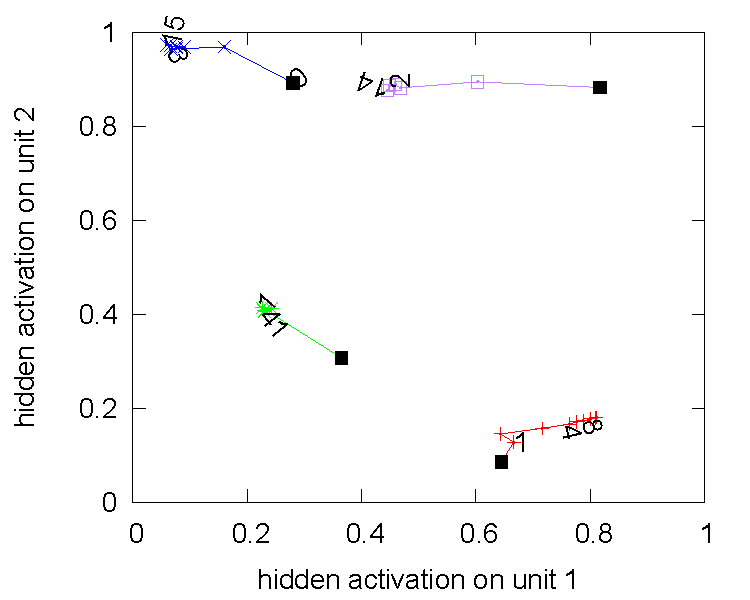
\includegraphics[width=0.48\textwidth]{img/hid-bal-good-convex.pdf}  \\
  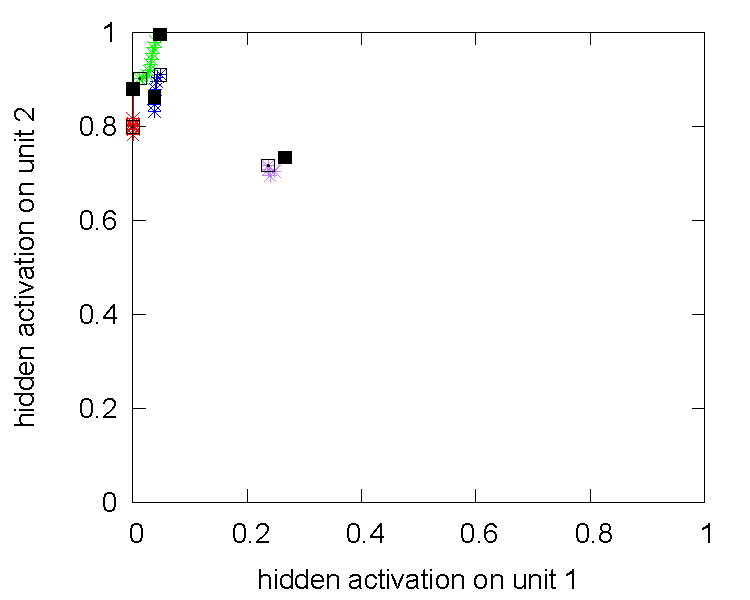
\includegraphics[width=0.48\textwidth]{img/hid-bal-good-step.pdf}  
  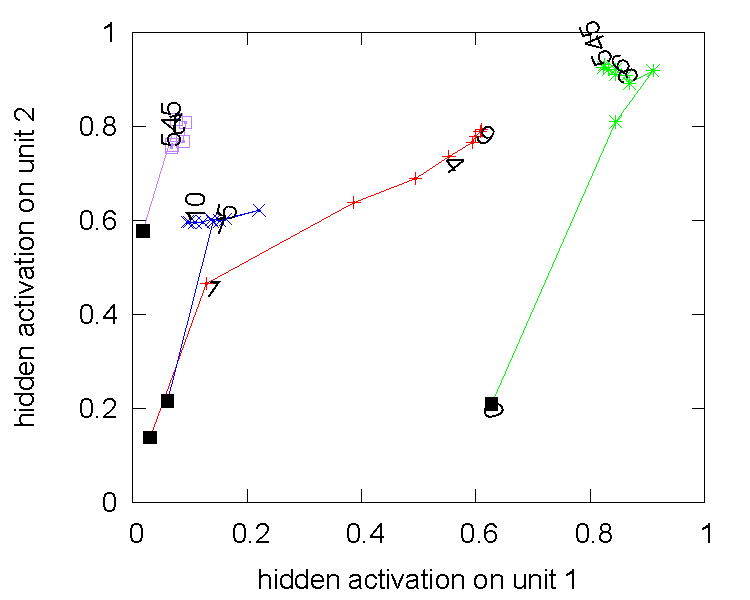
\includegraphics[width=0.48\textwidth]{img/hid-bal-good-stagnation.pdf}  \\ 
  \caption{\emph{BAL} hidden activations on the \emph{4-2-4 encoder}. Top $2\times2$ are {\bf un}successful networks and bottom $2\times2$ successful ones.}
  \label{fig:results-hidden-activations-bal}
\end{figure}

\begin{figure}[H]
  \centering
  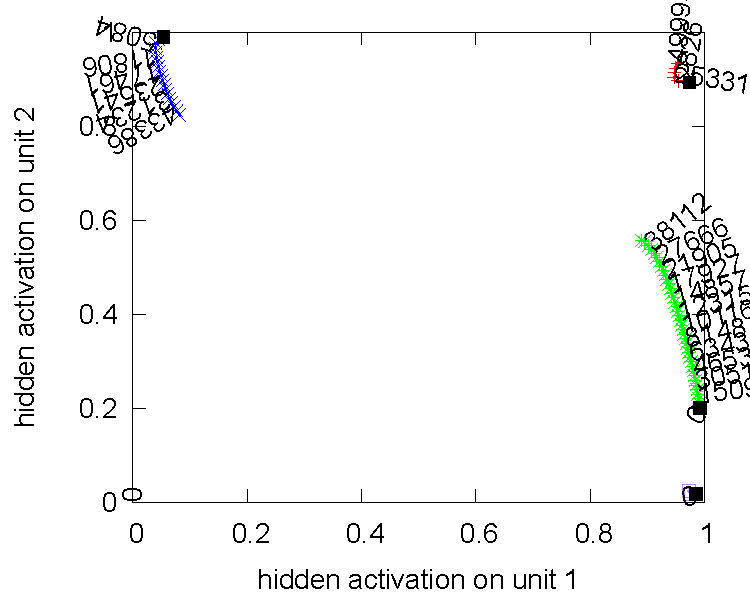
\includegraphics[width=0.48\textwidth]{img/hid-tlr-bad-static.pdf}  
  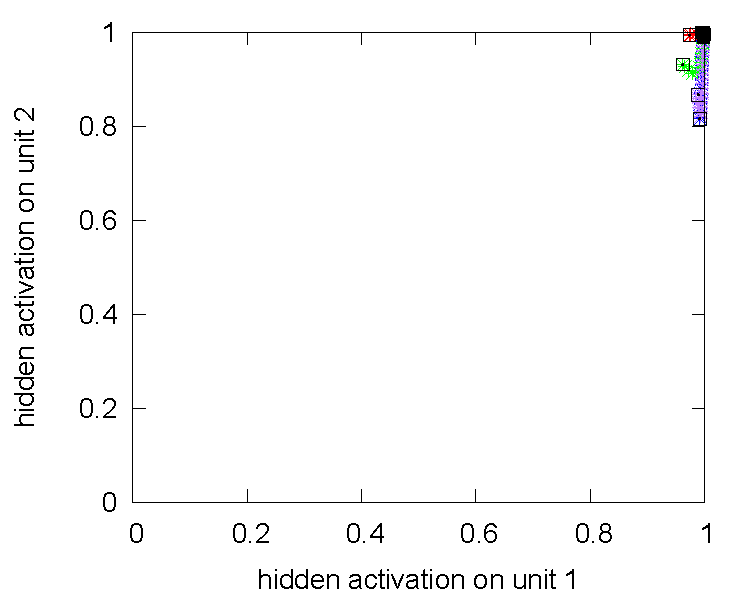
\includegraphics[width=0.48\textwidth]{img/hid-tlr-bad-tiny.pdf}  
  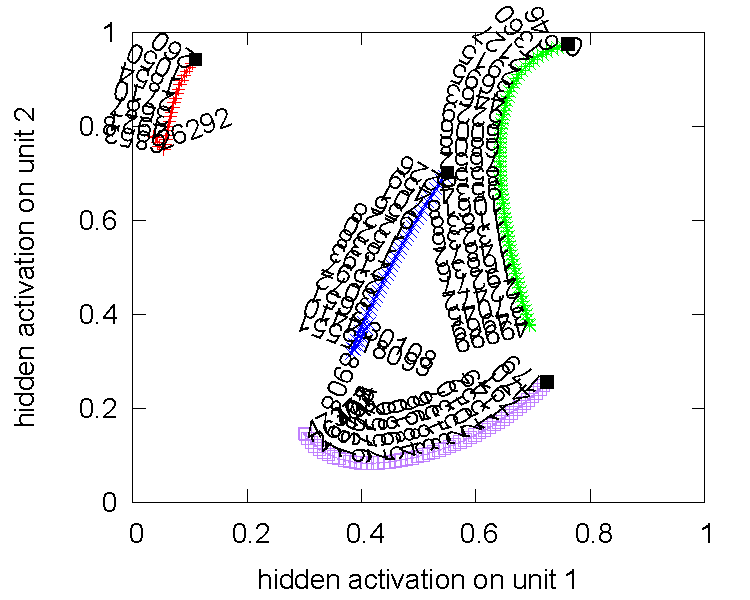
\includegraphics[width=0.48\textwidth]{img/hid-tlr-bad-init.pdf}  
  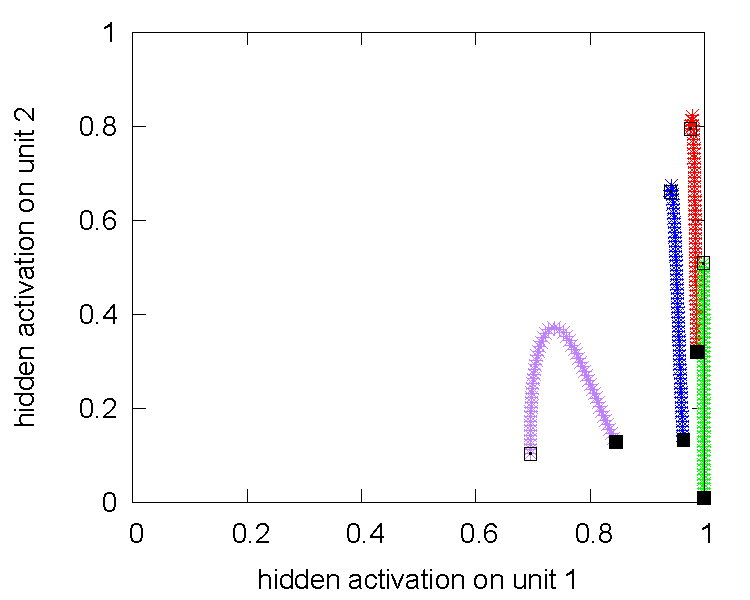
\includegraphics[width=0.48\textwidth]{img/hid-tlr-bad-weird.pdf}  
  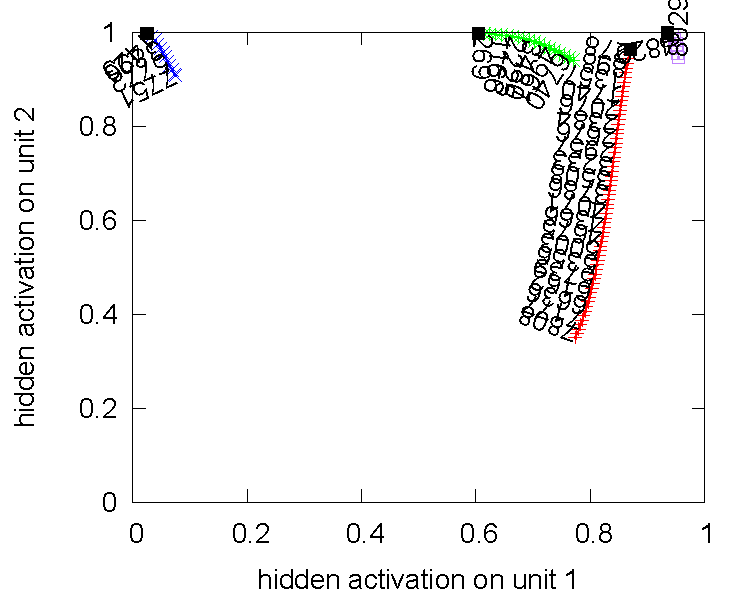
\includegraphics[width=0.48\textwidth]{img/hid-tlr-good-static.pdf}  
  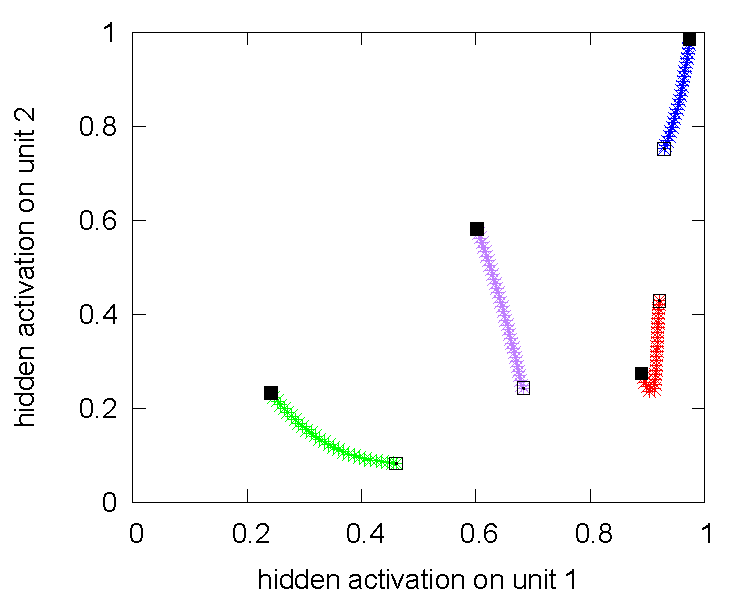
\includegraphics[width=0.48\textwidth]{img/hid-tlr-good-tiny.pdf}  
  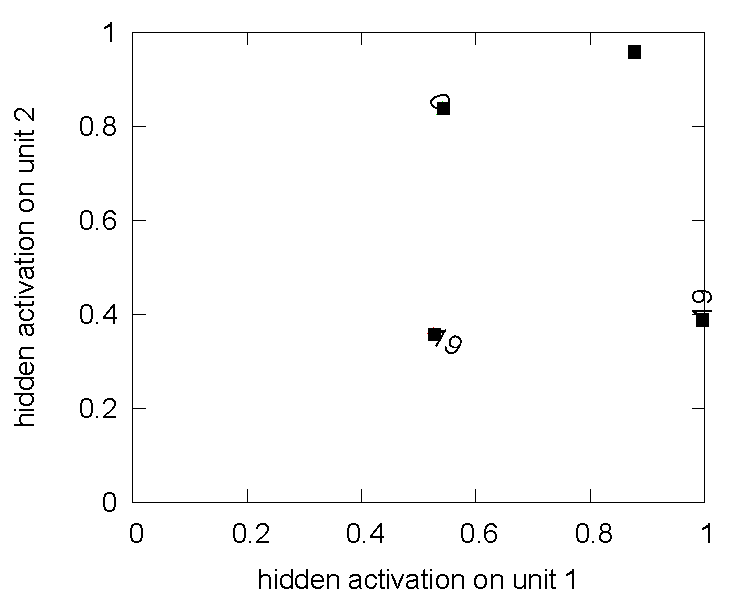
\includegraphics[width=0.48\textwidth]{img/hid-tlr-good-init.pdf}  
  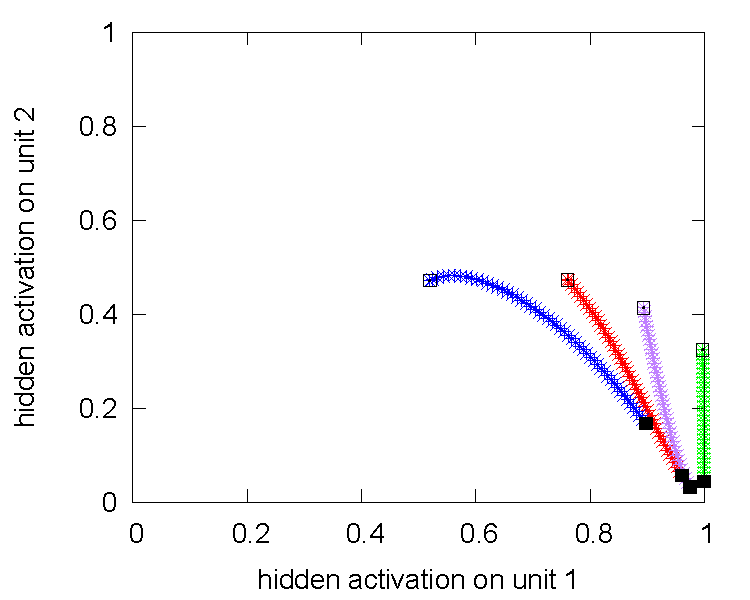
\includegraphics[width=0.48\textwidth]{img/hid-tlr-good-weird.pdf}  
  \caption{\emph{TLR} hidden activations on the \emph{4-2-4 encoder}. Top $2\times2$ are {\bf un}successful networks and bottom $2\times2$ successful ones.}
  \label{fig:results-hidden-activations-tlr}
\end{figure}

%============================================================
%\subsubsection{Features}

%==== TODO feature to epoch of best (in worst we will throw away) 


\subsubsection{Other} 

%======== (3D) L1 x L2 x epochs =========
%======== (3D) L1 x L2 x patSuccF =========
\begin{figure}[H]
  \centering
  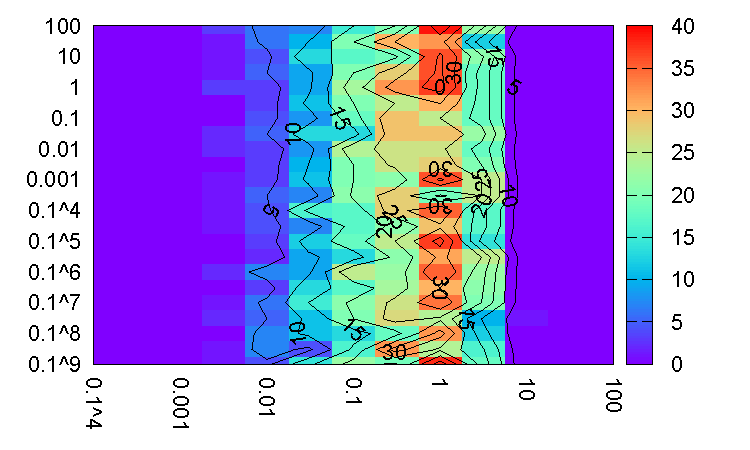
\includegraphics[width=0.48\textwidth]{img/bal-recirc-auto4-success.pdf}   
  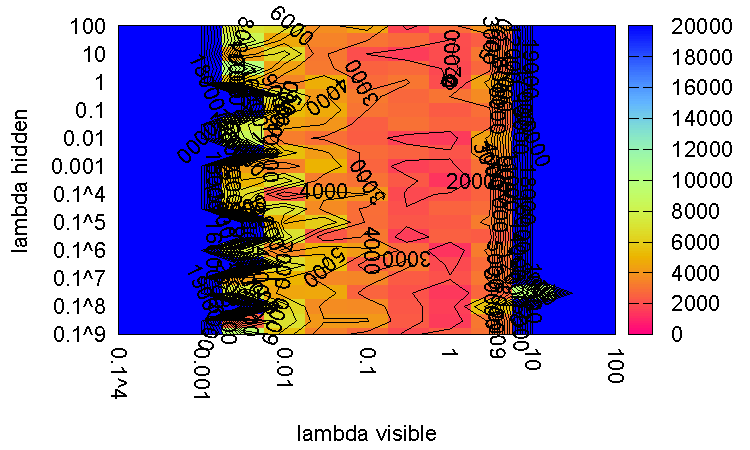
\includegraphics[width=0.48\textwidth]{img/bal-recirc-auto4-epoch.pdf}     
  \caption{BAL-recirc \ref{sec:our-bal-recirc} success and convergence on the \emph{4-2-4 Encoder} task with $\sigma = 2.3$ and $\mu = 0.0$.}
  \label{fig:results-bal-recirc-auto4-performance}
\end{figure}


%======== (3D) L1 x L2 x epochs =========
%======== (3D) L1 x L2 x patSuccF =========
\begin{figure}[H]
  \centering
  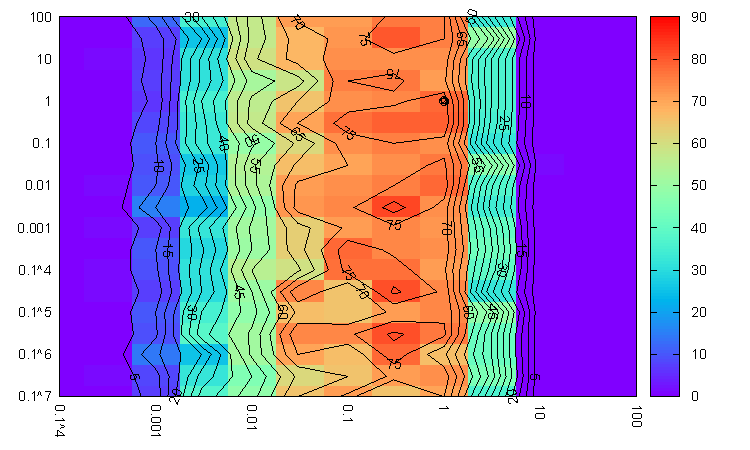
\includegraphics[width=0.48\textwidth]{img/generec-auto4-success.pdf}   
  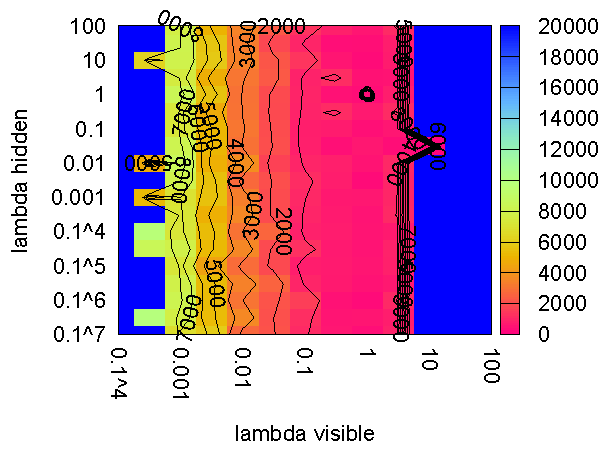
\includegraphics[width=0.48\textwidth]{img/generec-auto4-epoch.pdf}     
  \caption{GeneRec \ref{sec:models-generec} success and convergence on the \emph{4-2-4 Encoder} task with $\sigma = 2.3$ and $\mu = 0.0$.}
  \label{fig:results-generec-auto4-performance}
\end{figure}


